% Options for packages loaded elsewhere
\PassOptionsToPackage{unicode}{hyperref}
\PassOptionsToPackage{hyphens}{url}
%
\documentclass[
]{article}
\title{Market Forecasting Assignment: Multiple Linear Regression}
\author{Teacher: Dr.~Stefan Groesser, Dr.~Christoph Imboden}
\date{Autors: Benedech Rodolpho, Buehler Pascal, Geeler Ken 04.12.2021}

\usepackage{amsmath,amssymb}
\usepackage{lmodern}
\usepackage{iftex}
\ifPDFTeX
  \usepackage[T1]{fontenc}
  \usepackage[utf8]{inputenc}
  \usepackage{textcomp} % provide euro and other symbols
\else % if luatex or xetex
  \usepackage{unicode-math}
  \defaultfontfeatures{Scale=MatchLowercase}
  \defaultfontfeatures[\rmfamily]{Ligatures=TeX,Scale=1}
\fi
% Use upquote if available, for straight quotes in verbatim environments
\IfFileExists{upquote.sty}{\usepackage{upquote}}{}
\IfFileExists{microtype.sty}{% use microtype if available
  \usepackage[]{microtype}
  \UseMicrotypeSet[protrusion]{basicmath} % disable protrusion for tt fonts
}{}
\makeatletter
\@ifundefined{KOMAClassName}{% if non-KOMA class
  \IfFileExists{parskip.sty}{%
    \usepackage{parskip}
  }{% else
    \setlength{\parindent}{0pt}
    \setlength{\parskip}{6pt plus 2pt minus 1pt}}
}{% if KOMA class
  \KOMAoptions{parskip=half}}
\makeatother
\usepackage{xcolor}
\IfFileExists{xurl.sty}{\usepackage{xurl}}{} % add URL line breaks if available
\IfFileExists{bookmark.sty}{\usepackage{bookmark}}{\usepackage{hyperref}}
\hypersetup{
  pdftitle={Market Forecasting Assignment: Multiple Linear Regression},
  pdfauthor={Teacher: Dr.~Stefan Groesser, Dr.~Christoph Imboden},
  hidelinks,
  pdfcreator={LaTeX via pandoc}}
\urlstyle{same} % disable monospaced font for URLs
\usepackage[margin=1in]{geometry}
\usepackage{color}
\usepackage{fancyvrb}
\newcommand{\VerbBar}{|}
\newcommand{\VERB}{\Verb[commandchars=\\\{\}]}
\DefineVerbatimEnvironment{Highlighting}{Verbatim}{commandchars=\\\{\}}
% Add ',fontsize=\small' for more characters per line
\usepackage{framed}
\definecolor{shadecolor}{RGB}{248,248,248}
\newenvironment{Shaded}{\begin{snugshade}}{\end{snugshade}}
\newcommand{\AlertTok}[1]{\textcolor[rgb]{0.94,0.16,0.16}{#1}}
\newcommand{\AnnotationTok}[1]{\textcolor[rgb]{0.56,0.35,0.01}{\textbf{\textit{#1}}}}
\newcommand{\AttributeTok}[1]{\textcolor[rgb]{0.77,0.63,0.00}{#1}}
\newcommand{\BaseNTok}[1]{\textcolor[rgb]{0.00,0.00,0.81}{#1}}
\newcommand{\BuiltInTok}[1]{#1}
\newcommand{\CharTok}[1]{\textcolor[rgb]{0.31,0.60,0.02}{#1}}
\newcommand{\CommentTok}[1]{\textcolor[rgb]{0.56,0.35,0.01}{\textit{#1}}}
\newcommand{\CommentVarTok}[1]{\textcolor[rgb]{0.56,0.35,0.01}{\textbf{\textit{#1}}}}
\newcommand{\ConstantTok}[1]{\textcolor[rgb]{0.00,0.00,0.00}{#1}}
\newcommand{\ControlFlowTok}[1]{\textcolor[rgb]{0.13,0.29,0.53}{\textbf{#1}}}
\newcommand{\DataTypeTok}[1]{\textcolor[rgb]{0.13,0.29,0.53}{#1}}
\newcommand{\DecValTok}[1]{\textcolor[rgb]{0.00,0.00,0.81}{#1}}
\newcommand{\DocumentationTok}[1]{\textcolor[rgb]{0.56,0.35,0.01}{\textbf{\textit{#1}}}}
\newcommand{\ErrorTok}[1]{\textcolor[rgb]{0.64,0.00,0.00}{\textbf{#1}}}
\newcommand{\ExtensionTok}[1]{#1}
\newcommand{\FloatTok}[1]{\textcolor[rgb]{0.00,0.00,0.81}{#1}}
\newcommand{\FunctionTok}[1]{\textcolor[rgb]{0.00,0.00,0.00}{#1}}
\newcommand{\ImportTok}[1]{#1}
\newcommand{\InformationTok}[1]{\textcolor[rgb]{0.56,0.35,0.01}{\textbf{\textit{#1}}}}
\newcommand{\KeywordTok}[1]{\textcolor[rgb]{0.13,0.29,0.53}{\textbf{#1}}}
\newcommand{\NormalTok}[1]{#1}
\newcommand{\OperatorTok}[1]{\textcolor[rgb]{0.81,0.36,0.00}{\textbf{#1}}}
\newcommand{\OtherTok}[1]{\textcolor[rgb]{0.56,0.35,0.01}{#1}}
\newcommand{\PreprocessorTok}[1]{\textcolor[rgb]{0.56,0.35,0.01}{\textit{#1}}}
\newcommand{\RegionMarkerTok}[1]{#1}
\newcommand{\SpecialCharTok}[1]{\textcolor[rgb]{0.00,0.00,0.00}{#1}}
\newcommand{\SpecialStringTok}[1]{\textcolor[rgb]{0.31,0.60,0.02}{#1}}
\newcommand{\StringTok}[1]{\textcolor[rgb]{0.31,0.60,0.02}{#1}}
\newcommand{\VariableTok}[1]{\textcolor[rgb]{0.00,0.00,0.00}{#1}}
\newcommand{\VerbatimStringTok}[1]{\textcolor[rgb]{0.31,0.60,0.02}{#1}}
\newcommand{\WarningTok}[1]{\textcolor[rgb]{0.56,0.35,0.01}{\textbf{\textit{#1}}}}
\usepackage{graphicx}
\makeatletter
\def\maxwidth{\ifdim\Gin@nat@width>\linewidth\linewidth\else\Gin@nat@width\fi}
\def\maxheight{\ifdim\Gin@nat@height>\textheight\textheight\else\Gin@nat@height\fi}
\makeatother
% Scale images if necessary, so that they will not overflow the page
% margins by default, and it is still possible to overwrite the defaults
% using explicit options in \includegraphics[width, height, ...]{}
\setkeys{Gin}{width=\maxwidth,height=\maxheight,keepaspectratio}
% Set default figure placement to htbp
\makeatletter
\def\fps@figure{htbp}
\makeatother
\setlength{\emergencystretch}{3em} % prevent overfull lines
\providecommand{\tightlist}{%
  \setlength{\itemsep}{0pt}\setlength{\parskip}{0pt}}
\setcounter{secnumdepth}{-\maxdimen} % remove section numbering
\usepackage{amsmath}
\usepackage{placeins}
\usepackage{xcolor}
\ifLuaTeX
  \usepackage{selnolig}  % disable illegal ligatures
\fi

\begin{document}
\maketitle

\hypertarget{short-theory-recap-multiple-linear-regression-mlr}{%
\subsubsection{Short Theory Recap Multiple Linear Regression
(MLR)}\label{short-theory-recap-multiple-linear-regression-mlr}}

The model equation for MLR has the form \(y=X\Theta\) +\(\epsilon\)
,with \(y\) being the target vector, \(X\) the explanatory
Matrix,\(\Theta\) the parameter vector and the residuals with the
assumption that they are normally distributed \(\epsilon\)
\textasciitilde{} \(N(0,\sigma^{2})\). The estimation of \(\Theta\) is
done with the Maxium likelihood
\(L(\theta)=P(X|\theta)=\frac{1}{\sqrt(2\pi)\sigma}*e^{-\frac{1}{2\sigma^{2}}*||y-\theta X||^{2}}\)
by solving the equation \(\Theta=(X^{T}X)^{-1}X^{T}y\).

\hypertarget{dataset}{%
\subsubsection{Dataset}\label{dataset}}

The data from 7 common fish species for fishmarket is provided from
Kaggle.

\begin{figure}

{\centering 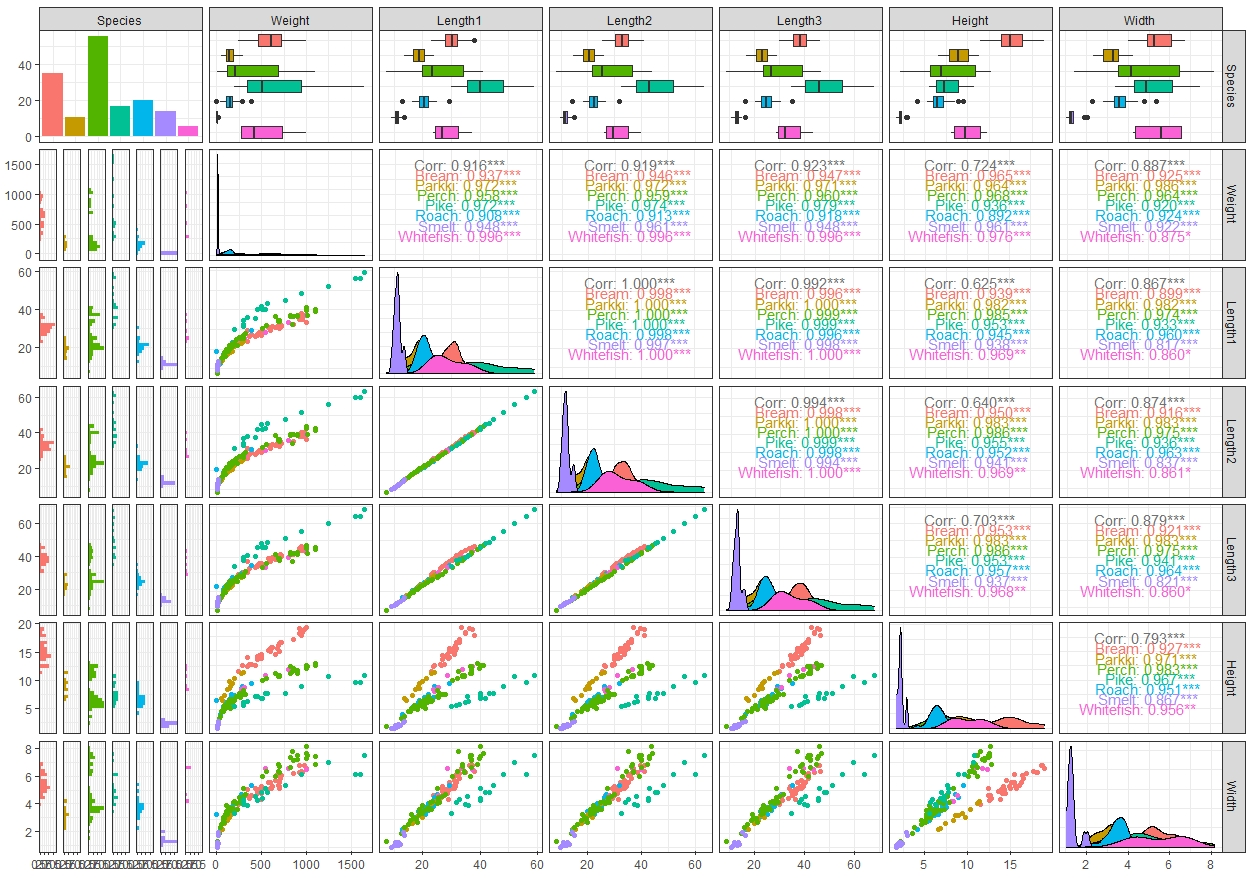
\includegraphics[width=0.95\linewidth]{fish_pairs} 

}

\caption{pairwise plot of the fish dataset}\label{fig:pairwise}
\end{figure}

\newpage
\usepackage[svgnames]{xcolor}

\#\definecolor{OliveGreen}{rgb}{91,179,0}

\hypertarget{data-exploration}{%
\subsubsection{Data exploration}\label{data-exploration}}

Information of the Dataset is gained with the following commands.

\begin{Shaded}
\begin{Highlighting}[]
\NormalTok{fish\_dat}\OtherTok{=}\NormalTok{readr}\SpecialCharTok{::}\FunctionTok{read\_csv}\NormalTok{(}\StringTok{"Fish.csv"}\NormalTok{)                        }\CommentTok{\#  reading as tibble}
\NormalTok{GGally}\SpecialCharTok{::}\FunctionTok{ggpairs}\NormalTok{(fish\_dat,}\FunctionTok{aes}\NormalTok{(}\AttributeTok{color =}\NormalTok{ Species)) }\SpecialCharTok{+} \FunctionTok{theme\_bw}\NormalTok{() }\CommentTok{\#  pairwise plot }
\FunctionTok{summary}\NormalTok{(fish\_dat);}\FunctionTok{str}\NormalTok{(fish\_dat);}\FunctionTok{View}\NormalTok{(fish\_dat)              }\CommentTok{\#  statistics and structure}
\end{Highlighting}
\end{Shaded}

The pairwise plot Figure \ref{fig:pairwise} provides a visual overview
of the dataset. It consists of 159 observations measured for 6 numerical
variables which measure properties of the fish and one categorical
variable to describe the Species. The coloring in the pairwise plot
allows a distinction of the Species, one can immediately observe that
the species \textcolor{lime}{Perch} has the most observations.

From the pairwise scatterplots a nonlinear relation between weight and
the other numerical variables is observed, therefore the correlation
\emph{cannot} be correctly interpreted with these variablepairs. Further
the other numerical variables are linearly correlated (the correlation
statistic can be interpreted), interestingly the 3 length measurements
have a very strong correlation to each other.The length of the fish is
measured in different ways, which is why there are three different
Length1 (vertical length), Length2 (diagonal length) and Length3 (cross
length).

The density plots helps see how the variables themselves are
distributed. For example the width of Smelt tends to have a bidmodal
distribution, altough this has to be taken with a grain of salt due to
the sparse data, see on the inverted histograms on the left. Also the
pairwise boxplots gives a good overview for comparison between the
different variables. For example it can be seen that the variance of the
species vary amongst the levels.

The distribution of the target variables is actually very important
since MLR assumes multivariate normality of the data, for other
distributions we might choose another model such as a
Generalized-Linear-Model to improve the model validity, but for this
analysis we stick to MLR.

\hypertarget{building-a-model}{%
\subsubsection{Building a Model}\label{building-a-model}}

To evaluate the accuracy of the model created in this chapter, the data
is split into a train and test set, using Simple Random Sampling without
Replacement (SRSWR). 80\% of the data is used for training and the
remaining 20\% is for testing prediction accuracy. The corresponding R
code is given below.

\begin{Shaded}
\begin{Highlighting}[]
\FunctionTok{set.seed}\NormalTok{(}\DecValTok{42}\NormalTok{);samp}\OtherTok{=} \FunctionTok{sample}\NormalTok{(}\DecValTok{1}\SpecialCharTok{:}\DecValTok{56}\NormalTok{,}\AttributeTok{size =} \DecValTok{11}\NormalTok{,}\AttributeTok{replace =}\NormalTok{ F)       }\CommentTok{\# Seed \& sample size 80\%}
\NormalTok{Perch\_train}\OtherTok{=}\NormalTok{Perch\_dat[}\SpecialCharTok{{-}}\NormalTok{samp,];Perch\_train}\OtherTok{=}\NormalTok{Perch\_dat[}\SpecialCharTok{{-}}\NormalTok{samp,] }\CommentTok{\# train / test sample}
\end{Highlighting}
\end{Shaded}

The dataset provides many different options to do linear regression,
nevertheless for MLR there is a problem with multicollinearity since a
lot of the variables are strongly correlated, meaning that if multiple
independent variables would be in the model it wouldn't be clear which
one explains the effect the best for the target variable.

Therefore the first thing we do is fitting a simple linear regression
model. We use the weight of a fish as a response variable. The
explanatory variable width is used, since this is intuitively a good
indicator for the weight of a fish from ``fishing experience''. In a
next step, we will also check whether a MLR model can represent the data
even better.

Finally, the models are compared quantitatively with the residual sum of
squares (RSS), R-squared and the Akaike information criterion (AIC).
Subsequently, the models will be used with the test set for predictions,
whose performance will be measured with the Mean Absolute
Deviation(MAD). The reason why we don't use Mean Squared Error(MSE) is
because of the small test set, one far point could massively influence
the statistic due to the square.

\hypertarget{simple-linear-regression}{%
\subsubsection{Simple linear
Regression}\label{simple-linear-regression}}

For a first approach we could just focus on the species Perch (in
swiss-german it's called Egli) since we have the most data there. Since
the weight hasn't got a linear relation to the other variables, we'll
have to transform it properly.

\begin{figure}

{\centering \includegraphics{Semestertask_Markfor_files/figure-latex/transformation-1} 

}

\caption{transformations of weight for Perch}\label{fig:transformation}
\end{figure}

If we transform the weight with the logarithm it looks a bit better but
still isn't linear see Figure \ref{fig:transformation}. The squareroot
transformation looks better, the data seems much more linearly
dependent.One can observe that the variance towards the right side of
the model increases even with after the transformations.

\begin{Shaded}
\begin{Highlighting}[]
\NormalTok{Perch\_fit}\OtherTok{=}\FunctionTok{lm}\NormalTok{(}\FunctionTok{sqrt}\NormalTok{(Weight)}\SpecialCharTok{\textasciitilde{}}\NormalTok{Width,}\AttributeTok{data =}\NormalTok{ Perch\_train) }\CommentTok{\#  Simple linear regression model}
\end{Highlighting}
\end{Shaded}

\begin{figure}

{\centering \includegraphics{Semestertask_Markfor_files/figure-latex/lm_perch-1} 

}

\caption{linear regression model for Perch weigth vs width}\label{fig:lm_perch}
\end{figure}

From the summary output we get the following model
\(Weight_{i}=(-6.000 + 4.9368 * Width_{i})^{2}\). The explained Variance
measurement \(R^{2}\) is with \(0.9683\) very high. the \(AIC\) for this
model is \(171.6\). The p-values for the both parameters hypothesis
tests are also significant. By inspecting the residuals in Figure
\ref{fig:resid_perch} we can check the model assumptions. The residuals
seem to follow a normal distribution, have constant mean and there are
no points which are crucial to shift the model. Nevertheless the
variance is not constant and increases towards the right side.

\begin{figure}

{\centering 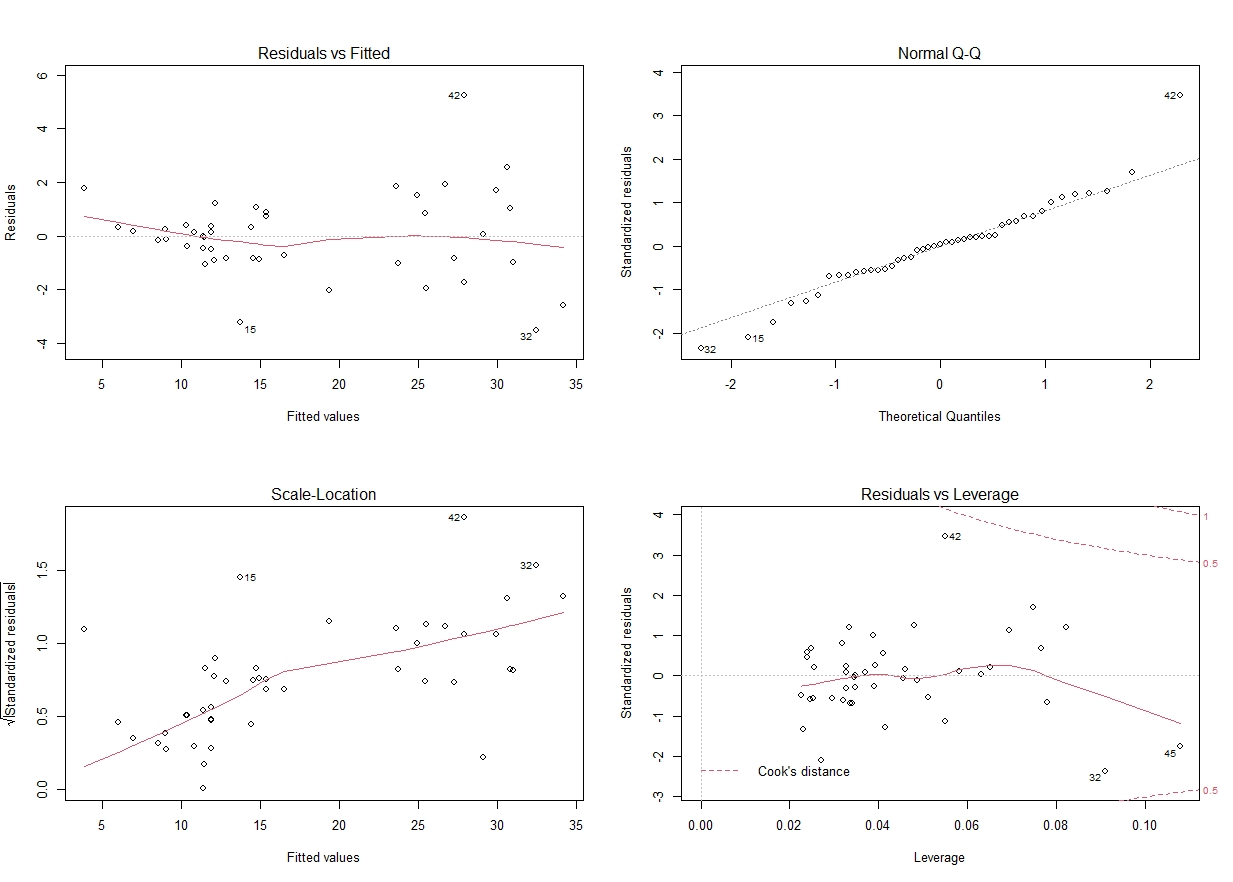
\includegraphics[width=0.8\linewidth]{Perch_res} 

}

\caption{Residuals for the Perchfit}\label{fig:resid_perch}
\end{figure}

~

The way we have chosen is starting with a sparse model. Lets make now a
full model and test if a larger model is more beneficial. The
multicollinearity is checked with Variance Inflation Factor and a F test
checks the importance of the variables

\begin{Shaded}
\begin{Highlighting}[]
\NormalTok{Perch\_fit\_full}\OtherTok{=}\FunctionTok{lm}\NormalTok{(}\FunctionTok{sqrt}\NormalTok{(Weight)}\SpecialCharTok{\textasciitilde{}}\NormalTok{.,}\AttributeTok{data =}\NormalTok{ Perch\_dat[,}\SpecialCharTok{{-}}\DecValTok{1}\NormalTok{]) }\CommentTok{\#  Multiple linear regression model}
\FunctionTok{summary}\NormalTok{(Perch\_fit\_full)}
\end{Highlighting}
\end{Shaded}

\begin{verbatim}
## 
## Call:
## lm(formula = sqrt(Weight) ~ ., data = Perch_dat[, -1])
## 
## Residuals:
##     Min      1Q  Median      3Q     Max 
## -1.5930 -0.6264 -0.0330  0.5929  2.5313 
## 
## Coefficients:
##             Estimate Std. Error t value Pr(>|t|)    
## (Intercept)  -7.0051     0.6527 -10.733 1.41e-14 ***
## Length1       0.4430     0.6227   0.711 0.480156    
## Length2      -0.5321     0.9527  -0.558 0.579014    
## Length3       0.4118     0.6465   0.637 0.527082    
## Height        1.1788     0.3228   3.652 0.000622 ***
## Width         1.3754     0.3956   3.477 0.001059 ** 
## ---
## Signif. codes:  0 '***' 0.001 '**' 0.01 '*' 0.05 '.' 0.1 ' ' 1
## 
## Residual standard error: 0.9372 on 50 degrees of freedom
## Multiple R-squared:  0.9896, Adjusted R-squared:  0.9885 
## F-statistic: 947.4 on 5 and 50 DF,  p-value: < 2.2e-16
\end{verbatim}

\begin{Shaded}
\begin{Highlighting}[]
\NormalTok{car}\SpecialCharTok{::}\FunctionTok{vif}\NormalTok{(Perch\_fit\_full)}
\end{Highlighting}
\end{Shaded}

\begin{verbatim}
##    Length1    Length2    Length3     Height      Width 
## 1780.07795 4626.41486 2376.77263   54.03761   30.85782
\end{verbatim}

\begin{Shaded}
\begin{Highlighting}[]
\FunctionTok{drop1}\NormalTok{(Perch\_fit\_full)}
\end{Highlighting}
\end{Shaded}

\begin{verbatim}
## Single term deletions
## 
## Model:
## sqrt(Weight) ~ Length1 + Length2 + Length3 + Height + Width
##         Df Sum of Sq    RSS     AIC
## <none>               43.916 -1.6126
## Length1  1    0.4445 44.360 -3.0487
## Length2  1    0.2739 44.190 -3.2644
## Length3  1    0.3563 44.272 -3.1601
## Height   1   11.7162 55.632  9.6306
## Width    1   10.6182 54.534  8.5143
\end{verbatim}

The VIF helps us to identify multicollinearity and indicates that the
variables have a very high collinearity as expected. Especially the
three variables of the lengths result in massively higher VIF values
than for the other variables.

\end{document}
